\section{Inverting learned diffusion steps}
\label{sec:experiment}
\begin{figure*}[t]
\centering
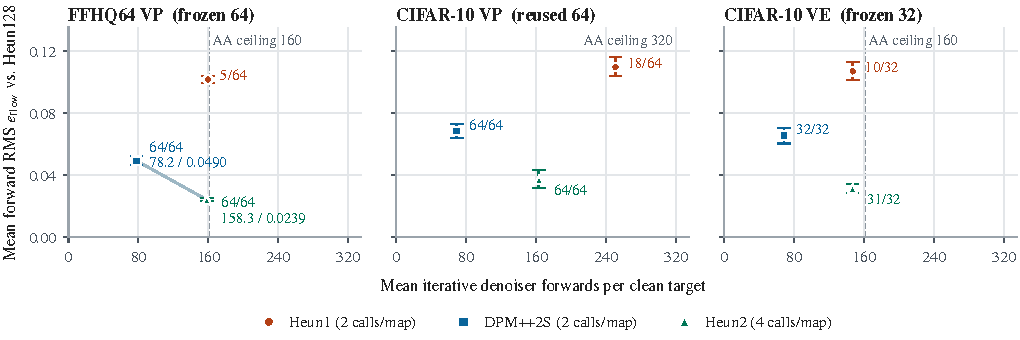
\includegraphics[width=\textwidth]{../figures/tradeoff.pdf}
\caption{\textbf{Two FFHQ64 choices recover the same clean sources.}
DPM++2S uses fewer inverse calls and Heun2 gives lower forward RMS. Marker labels give clean recovery counts. The two linked points also give mean iterative forwards and forward RMS. Bars show 95\% seed-bootstrap intervals for mean forward RMS against Heun128. The panels share axes but use the indicated cohort-specific ceilings. The reused primary panel has saved GPU targets and a CPU inverse. The separately frozen FFHQ64 and VE panels use CPU targets and inverses. \Cref{tab:recovery} includes noisy targets and the other primary maps.}
\label{fig:tradeoff}
\end{figure*}

\begin{table*}[t]
\centering\small
\setlength{\tabcolsep}{7pt}
\begin{tabular}{@{}lrrrrr@{}}
\toprule
Step map & Calls per map & Clean recovered & Noisy recovered & Mean $e_{\rm flow}$ & Mean clean $N_f$\\
\midrule
\multicolumn{6}{@{}l}{\textbf{FFHQ64 VP} \enspace \FFHQN{} separately frozen sources, \FFHQCap{} forwards, CPU targets}\\
\tablerows{generated/ffhq_rows_labeled}
\midrule
\multicolumn{6}{@{}l}{\textbf{CIFAR-10 VP} \enspace \PrimaryN{} reused sources, \PrimaryCap{} forwards, saved GPU targets}\\
\tablerows{generated/primary_rows_labeled}
\midrule
\multicolumn{6}{@{}l}{\textbf{CIFAR-10 VE} \enspace \VEN{} separately frozen sources, \FFHQCap{} forwards, CPU targets}\\
\tablerows{generated/ve_rows_labeled}
\bottomrule
\end{tabular}
\caption{\textbf{Anderson recovery at each cohort's registered ceiling.}
Recovery requires source RMS $e_x\le0.02$. $N_f$ counts iterative denoiser forwards. Each inverse has two initializer calls, with final diagnostics also accounted for separately. The forward reference is Heun128 on the target-generation device. Supplement~E reports source errors, residuals and hybrid work.}
\label{tab:recovery}
\end{table*}

We now treat the denoisers as fixed neural networks. The inverse sees $y=F(x)+\eta$, the operator $F$ and its schedule. It starts at a two-step reverse Euler estimate computed from $y$. Source truth, the seed, intermediate states and the clean version of a noisy target are held by the evaluator. With $\rms(v)=\|v\|_2/\sqrt d$ over the $d$ image coordinates, we measure
\begin{equation}
 \begin{aligned}
 e_x&=\rms(\widehat x-x),& e_y&=\rms(F(\widehat x)-y),\\
 e_{\rm flow}&=\rms(F(x)-F_{\rm ref}(x)).&&
 \end{aligned}
 \label{eq:metrics}
\end{equation}
A recovery has $e_x\le0.02$. The inverse selects by $e_y$, using a residual stopping tolerance of $2\times10^{-6}$. Clean targets have $\eta=0$. Noisy targets use Gaussian noise with coordinate standard deviation $10^{-3}$, paired across maps at each source.

\paragraph{Sources and maps.}
We use the public unconditional EDM CIFAR-10 VP, CIFAR-10 VE and FFHQ64 VP checkpoints~\cite{karras2022,cifar2009,karras2019}. Each source is the state at sigma 2 after Heun64 from sigma 80, initialized with $80$ times a seeded standard Gaussian array. The test interval is $2\to1/8$. We compare two Euler steps, one Heun step, one sigma-midpoint step, one DPM++2S step, and two Heun steps. Two-step grids use EDM's fixed sigma-power schedule with exponent 7. A repeated primary diagnostic also uses the geometric Heun4 grid from \cref{cor:schedule}. The numerical forward reference is Heun128 on the same network and interval. We report its disagreement with Heun64 as a refinement check.

\paragraph{Cohorts and precision.}
The primary \PrimaryN{} CIFAR-VP sources were already observed before the frozen comparison. Their saved targets are from GPU execution and their inverses run on CPU. The fresh \VEN{} CIFAR-VE and \FFHQN{} FFHQ64-VP seeds were frozen separately after disjoint development runs. Their targets and inverses use the same CPU operator. Outer states are float64 and denoisers evaluate in float32. A clean CPU-target replay on the reused primary cohort isolates the effect of the device change. Each inverse runs on one image at a time. The independently seeded source is the unit of analysis. All method, noise and budget comparisons within a cohort are paired by seed.

\paragraph{Inverses and work.}
Anderson acceleration (AA)~\cite{walker2011} extrapolates the target-residual fixed-point map with memory five and damping $0.8$. Two primary controls start from the observed AA iterate available within 80 forwards and continue with L-BFGS~\cite{liu1989} or inexact Newton--GMRES~\cite{saad1986}. The L-BFGS control charges line searches and gradient traversals. Newton--GMRES charges centered finite-difference Jacobian actions, line searches and unfinished work. Primary ceilings are 80, 160 and \PrimaryCap{} iterative denoiser traversals. Each charges forward and backward traversals, including the shared AA warm work for each hybrid. The fresh cohorts use AA with a ceiling of \FFHQCap{} forwards. A forward pass through the \emph{step map} can call the denoiser more than once. We report these calls per map separately from the inverse's actual iterative work, and itemize initialization and final diagnostics in the supplement.

\paragraph{Uncertainty.}
Failure intervals use two-sided exact binomial limits. Mean and paired-difference intervals use 10,000 bootstrap draws of source seeds, with the same resampled indices on both sides of a contrast. Cohorts are summarized separately.
